\documentclass[sigconf, nonacm=true, screen=true]{acmart}
\usepackage{listings}

\begin{document}

\title{CPE480 Assignment 3: Pipelined Tangled }
\subtitle{Implementor's Notes}

\author{Cain Hubbard}
\author{Collin Lebanik}
\author{Nick Santini}
\author{Tristan Barnes}
\affiliation{%
    \department{Department of Electrical and Computer Engineering}
    \institution{University of Kentucky}
    \city{Lexington}
    \state{Kentucky}
    \country{United States}
}


\begin{abstract}
This is an pipelined implementation of a processor for the Tangled instruction set.
\end{abstract}


\maketitle


\section{General Approach}

Our AIK specification of Tangled is largely based on team 24's specification. See the Appendix \ref{appendix:encodings} for the AIK specification. 

We designed an ALU which would instantiate all the floating point operations. This would be done by making a call to the floating point instructions that we were given in the last assignment with some few changes. For this project we added NAN support for all of the floating point operations. Along with instantiating all of the floating operations our ALU also assigned the output based on the operation.  

We broke our pipeline down into 4 stages inside one module called tangled. The names of the stages are as follows: Load, Decode, Execute, and Write-back. The first stage is the load stage which is used to determine where the instruction is coming from, either the pc or a branch instruction. Inside the load stage there are some functions that are used to determine if the instruction  is a sys and a qat instruction which will be handled differently. The next stage in our pipeline is the decoding stage. This stage is used to determine what type of instruction is being used and it is figured out by using a bunch of functions to determine what instruction is being called. Value forwarding is also implemented inside the decoding stage. The next stage is the execute stage. This is where it is determined if a branch should be taken or not and where to go if the branch is taken. The writeback value is also determined in this stage. Lastly if a branch is taken then a bubble is implemented into the pipeline. The last stage in our pipeline is the writeback stage. This is where the writeback value is written into the regfile.

As recommended by Dr. Dietz, we made use of Verilog's \texttt{`define}s to name ranges of bits we frequently use and the OP code for each instruction.

We decided to run our Verilog locally, so a few commands differ from Dr. Dietz's web interface. A Makefile is included to facilitate running the project. To run different assembly programs, the \texttt{readmemh} instructions must be changed to the appropriate filenames.


\section{Testing}
Our testing consisted of carefully chosen test code that would cover most of the Verilog that we wrote. Our testbench includes a dumpfile macro with dumpvars that include the registers and wires we used in our Tangled module. Using the dumpfile along with those dumpvars allowed us to debug most of our program with the program GTKWave. With GTKWave, we could see the instructions and values in the order they were being executed, which when following along with the test assembly output from AIK, allowed us to follow the program and ensure our instructions were handled properly. Our Makefile, along with the testbench we created, allows us to use a macro that includes every test assembly file ending in \texttt{.tasm} that we created in order to produce dump files for all of our test cases at once. This allows us to view each of the different outputs for each of the given test cases in GTKWave individually. This means that the testbench does not need to be modified to run each of the different test assembly files.


Testing the Qat instructions is the most simple and straight forward of all of the instructions to test. This is because the Qat instructions are required to be trapped like a sys call. If the program halts after the specified Qat instruction then we know that it passed. Non-Qat instructions were added after the Qat instructions during testing to ensure that the program was actually halting and not just reaching the sys call at the end of our assembly instructions. Each of the different Qat instructions were given their own test assembly file. In order to run the specific Qat instruction, the GTKWave command along with the name of the specific Qat assembly dumpfile can be run. An example of the that would be:

\begin{lstlisting}[language=bash]
$ gtkwave testing/qatOr.vcd
\end{lstlisting}


\section{Issues}

We ran into an issue with our value forwarding. If there was an instruction, say \texttt{add} after a branch, if the branch was taken then the \texttt{add} would not be executed (more specifically, the ALU add would be performed, but the value would not be written back to the register file). However, Since the \texttt{add} remains in the pipeline, any instruction that followed the branch's jump and used the register that the \texttt{add} would have written to would identify the \texttt{add} further down the pipeline and attempt to apply value-forwarding to use the result of that \texttt{add} instead of the current value for that register in the register file. This issue was resolved by applying an extra condition to our value-forwarding logic that ensured that the value being forwarded had not been "aborted". 

The next issue was with our copy instruction. We ran into an issue where our values were not being copied right and we ran into an instance where we had an infinite loop. The issue was that our copy instruction was writing back the wrong value. It was writing back the Rd value instead of the intended Rs value so we made a change to correct that.


\clearpage
\appendix


\section{Encodings} 
\label{appendix:encodings}
The instructions are divided into five different encoding formats, named Format 0 - 4, based on the number and bit-length of operands. Bit 15, named \texttt{frmtA}, specifies whether an instruction follows Format 0 or one of the other four formats by 1 and 0, respectively. Each of the remaining four formats are distinguished by the value specified by the bitfield 14 and 13, named \texttt{frmtB}. \textit{Table \ref{table:frmtB-encodings}} presents the \texttt{frmtB} encodings.

\begin{center}
    \begin{table}[h]
        \begin{tabular}{cc}
            \toprule
            \texttt{frmtB} Encoding & Instruction Format \\
            \midrule
            \texttt{01} & Format 1 \\
            \texttt{10} & Format 2 \\
            \texttt{11} & Format 3 \\
            \texttt{00} & Format 4 \\
            \bottomrule
        \end{tabular}
        \caption{\texttt{frmtB} Encodings}
        \label{table:frmtB-encodings}
    \end{table}
\end{center}


\subsection{Format 0}
Instructions encoded with Format 0 (i.e. \texttt{frmtA} = \texttt{1}) contain a 4-bit operand, an 8-bit operand, and a 3-bit function code, named \texttt{func0}, that specifies the function of the instruction. The 4-bit operand is located in bits 12 - 9 and may specify one of the 16 main processor registers or a 4-bit immediate value, depending on the instruction. The 8-bit operand is located in bits 7 - 0 and may specify an 8-bit immediate value, an 8-bit PC-offset, or one of the 256 Qat coprocessor registers, depending on the instruction. The two most significant bits of \texttt{func0} are located in bits 14 and 13 and the least significant bit is located in bit 8. The \texttt{func0} bitfield is split up in order to allow the first 4-bit and first 8-bit operands in each format to be placed in the same location. This aids in simplifying microarchitecture design. \textit{Figure \ref{figure:format0-bitfields}} presents the Format 0 bitfields. \textit{Table \ref{table:func0-encodings}} presents the \texttt{func0} encodings. 

\begin{figure}[h]
    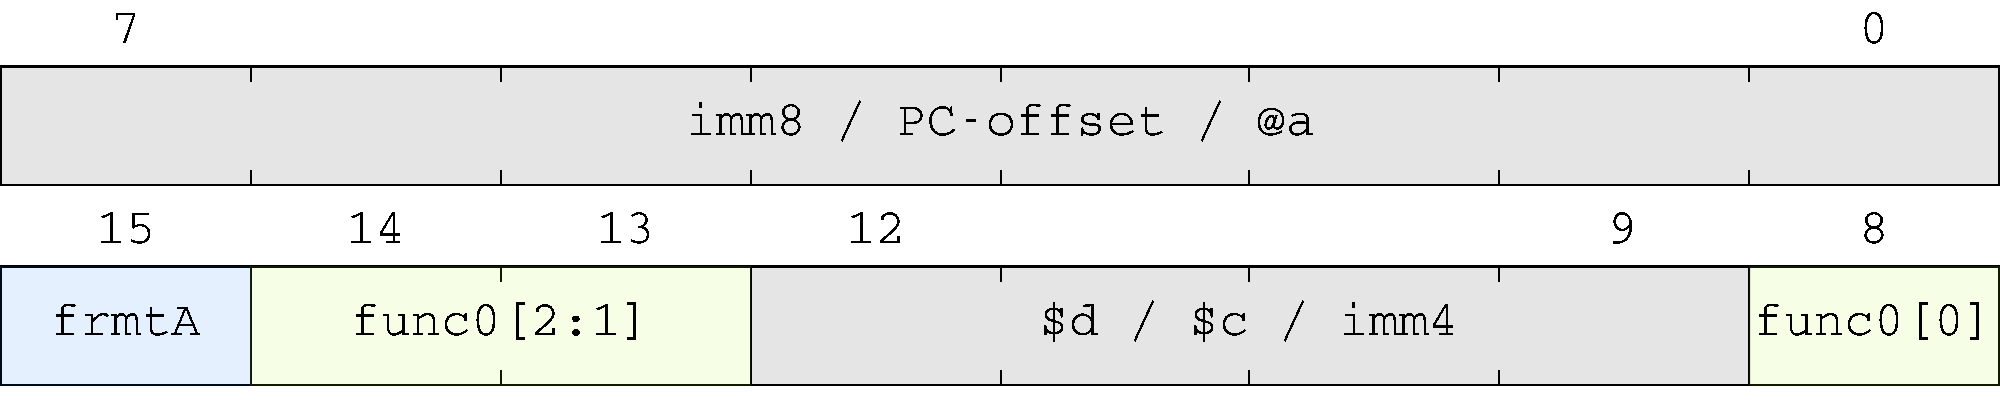
\includegraphics[width=\columnwidth]{bitfields/format0_2-lane.pdf}
    \caption{Format 0 Bitfields}
    \label{figure:format0-bitfields}
\end{figure}

\begin{center}
    \begin{table}[h]
        \begin{tabular}{cc}
            \toprule
            \texttt{func0} Encoding & Instruction \\
            \midrule
            \texttt{0x0} & \texttt{lex} \\
            \texttt{0x1} & \texttt{lhi} \\
            \texttt{0x2} & \texttt{brf} \\
            \texttt{0x3} & \texttt{brt} \\
            \texttt{0x4} & \texttt{meas} \\
            \texttt{0x5} & \texttt{next} \\
            \texttt{0x6} & \texttt{had} \\
            \texttt{0x7} & \textit{Undefined} \\
            \bottomrule
        \end{tabular}
        \caption{\texttt{func0} Encodings}
        \label{table:func0-encodings}
    \end{table}
\end{center}


\subsection{Format 1}
Instructions encoded with Format 1 (i.e. \texttt{frmtA} = \texttt{0}, \texttt{frmtB} = \texttt{1}) contain two 4-bit operand bitfields and a 5-bit function code, named \texttt{func1}, that specifies the function of the instruction. The first 4-bit operand is located in bits 12 - 9 and specifies a main processor register, which is the instruction's destination register if it contains two operands, otherwise it is simply the instruction's sole operand. The second 4-bit operand is located in bits 3 - 0 and specifies the instruction's second main processor register operand if the instruction contains two operands, otherwise the value is treated as a "don't care" and may hold an arbitrary value. (The assembler defaults to a second operand value of all zeros for such single-operand instructions). The \texttt{func1} bitfield is located in bits 8 - 4. \textit{Figure \ref{figure:format1-bitfields}} presents the Format 1 bitfields. \textit{Table \ref{table:func1-encodings}} presents the \texttt{func1} encodings. Notice that ALU and non-ALU Format 1 instructions can be easily distinguished by the MSB of the \texttt{func1} field. 

\begin{figure}[h]
    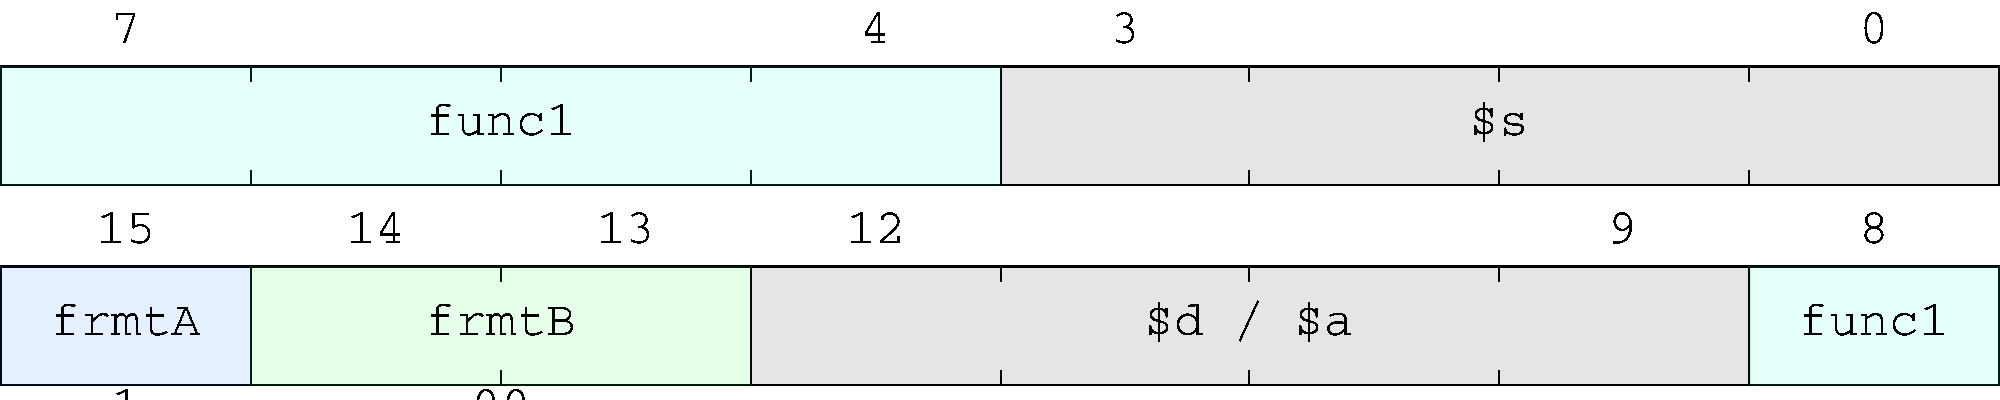
\includegraphics[width=\columnwidth]{bitfields/format1_2-lane.pdf}
    \caption{Format 1 Bitfields}
    \label{figure:format1-bitfields}
\end{figure}

\begin{center}
    \begin{table}[h]
    	\begin{tabular}[t]{cc}
            \toprule
            \texttt{func1} & Instruction \\
            \midrule
            \texttt{0x00} & \texttt{not} \\
            \texttt{0x01} & \texttt{float} \\
            \texttt{0x02} & \texttt{int} \\
            \texttt{0x03} & \texttt{neg} \\
            \texttt{0x04} & \texttt{negf} \\
            \texttt{0x05} & \texttt{recip} \\
            \texttt{0x06} & \texttt{add} \\
            \texttt{0x07} & \texttt{mul} \\
            \texttt{0x08} & \texttt{slt} \\
            \texttt{0x09} & \texttt{and} \\
            \texttt{0x0A} & \texttt{or} \\
            \texttt{0x0B} & \texttt{shift} \\
            \texttt{0x0C} & \texttt{xor} \\
            \texttt{0x0D} & \texttt{addf} \\
            \texttt{0x0E} & \texttt{mulf} \\
            \texttt{0x0F} & \texttt{sltf} \\
            \bottomrule
        \end{tabular}
    	\begin{tabular}[t]{cc}
            \toprule
            \texttt{func1} & Instruction \\
            \midrule
            \texttt{0x10} & \texttt{jumpr} \\
            \texttt{0x11} & \textit{Undefined} \\
            \(\cdot\) & \(\cdot\) \\
            \(\cdot\) & \(\cdot\) \\
            \(\cdot\) & \(\cdot\) \\
            \(\cdot\) & \(\cdot\) \\
            \(\cdot\) & \(\cdot\) \\
            \texttt{0x17} & \textit{Undefined} \\
            \texttt{0x18} & \texttt{load} \\
            \texttt{0x19} & \texttt{store} \\
            \texttt{0x1A} & \texttt{copy} \\
            \texttt{0x1B} & \textit{Undefined} \\
            \(\cdot\) & \(\cdot\) \\
            \(\cdot\) & \(\cdot\) \\
            \(\cdot\) & \(\cdot\) \\
            \texttt{0x1F} & \textit{Undefined} \\
            \bottomrule
        \end{tabular}
        \caption{\texttt{func1} Encodings}
        \label{table:func1-encodings}
    \end{table}
\end{center}


\subsection{Format 2}
Instructions encoded with Format 2 (i.e. \texttt{frmtA} = \texttt{0}, \texttt{frmtB} = \texttt{2}) contain a single 8-bit operand and a 5-bit function code, named \texttt{func2}, that specifies the function of the instruction. The 8-bit operand, which specifies a Qat register in all instructions, is located in bits 7 - 0. The \texttt{func2} bitfield is located in bits 12 - 8. \textit{Figure \ref{figure:format2-bitfields}} presents the Format 2 bitfields. \textit{Table \ref{table:func2-encodings}} presents the \texttt{func2} encodings. 

\begin{figure}[h]
    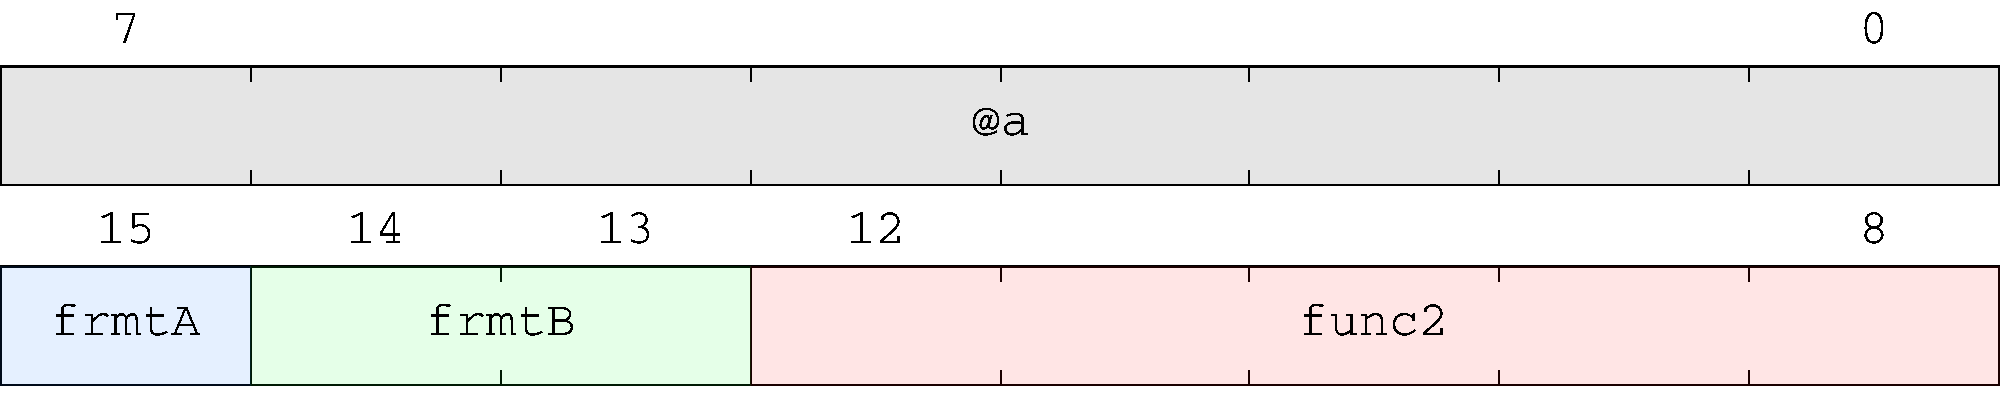
\includegraphics[width=\columnwidth]{bitfields/format2_2-lane.pdf}
    \caption{Format 2 Bitfields}
    \label{figure:format2-bitfields}
\end{figure}

\begin{center}
    \begin{table}[h]
        \begin{tabular}{cc}
            \toprule
            \texttt{func2} Encoding & Instruction \\
            \midrule
            \texttt{0x00} & \texttt{one} \\
            \texttt{0x01} & \texttt{zero} \\
            \texttt{0x02} & \texttt{not} \\
            \texttt{0x03} & \textit{Undefined} \\
            \(\cdot\) & \(\cdot\) \\
            \texttt{0x1F} & \textit{Undefined} \\
            \bottomrule
        \end{tabular}
        \caption{\texttt{func2} Encodings}
        \label{table:func2-encodings}
    \end{table}
\end{center}


\subsection{Format 3}
Instructions encoded with Format 3 (i.e. \texttt{frmtA} = \texttt{0}, \texttt{frmtB} = \texttt{3}) contain three 8-bit, Qat register, operand bitfields and a 5-bit function code, named \texttt{func3}, that specifies the function of the instruction. Format 3 instructions are the only 2-word (i.e. 32-bit) instructions in the Tangled ISA. The first operand is located in bits 7 - 0, the second in bits 23 - 16, and the third in bits 31 - 24. For instructions with only two operands, the third operand is treated as a "don't care" and may hold an arbitrary value. (The assembler defaults to a third operand value of all zeros for such two-operand instructions). The \texttt{func3} bitfield is located in bits 12 - 8. \textit{Figure \ref{figure:format3-bitfields}} presents the Format 3 bitfields. Notice that the destination or single Qat register operand is aligned across Formats 0, 2, and 3. \textit{Table \ref{table:func3-encodings}} presents the \texttt{func3} encodings. Notice that double- and triple-operand Format 3 instructions can be easily distinguished by the MSB of the \texttt{func3} field. 

\begin{figure}[h]
    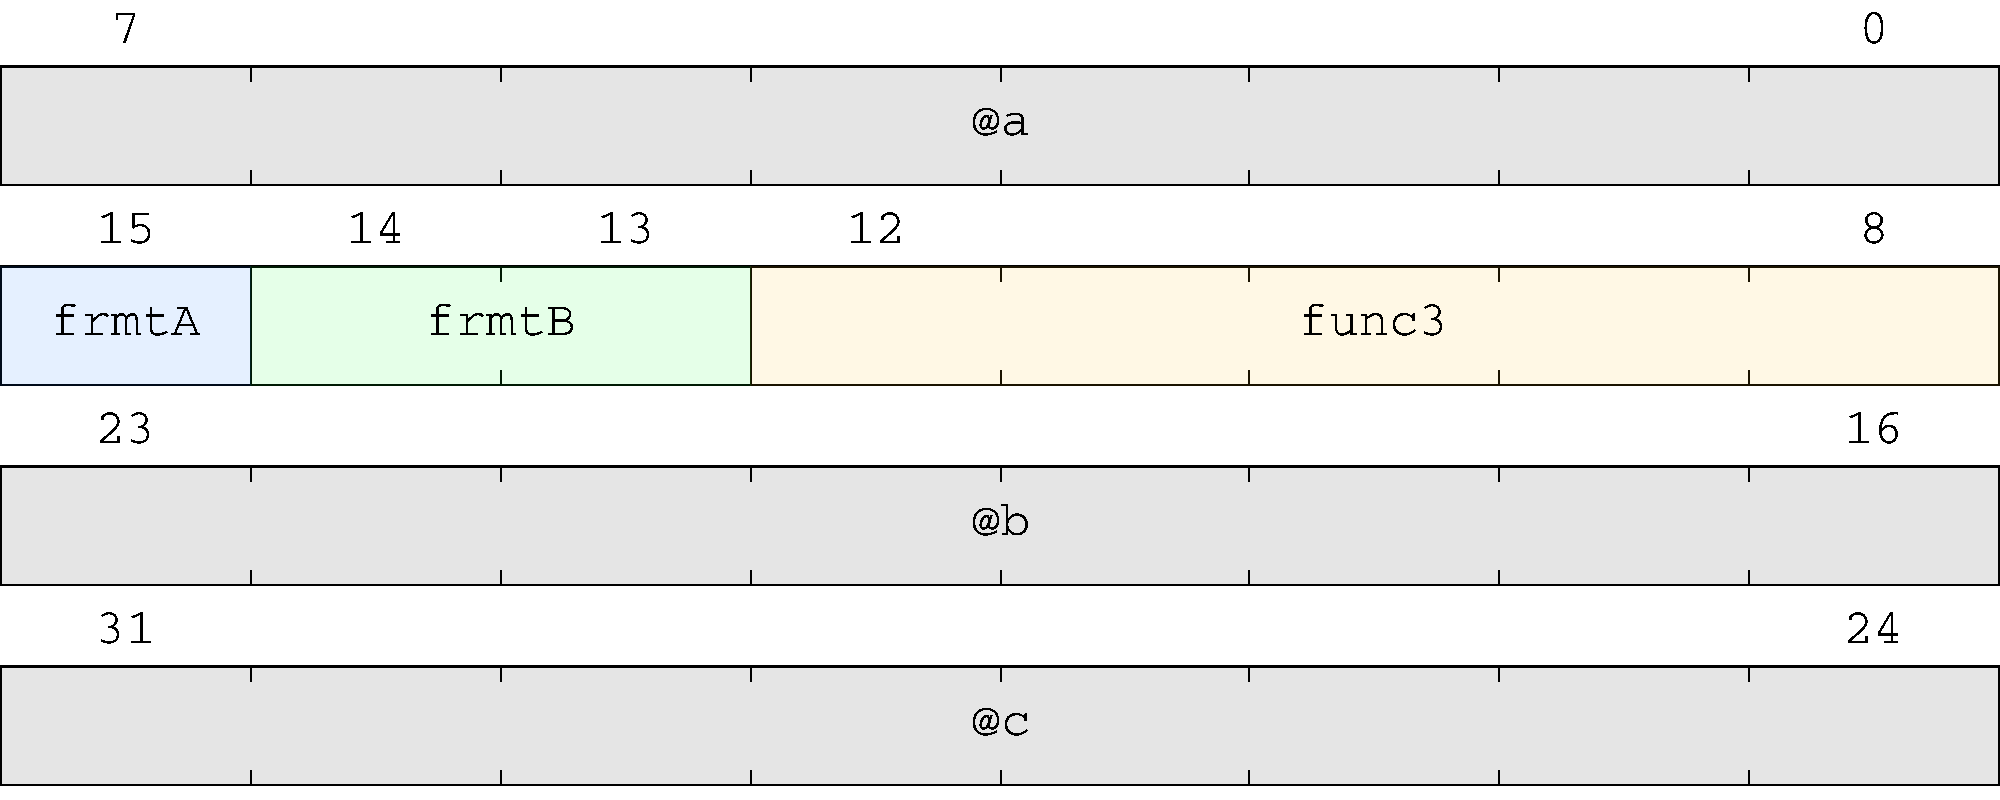
\includegraphics[width=\columnwidth]{bitfields/format3_2-lane.pdf}
    \caption{Format 3 Bitfields}
    \label{figure:format3-bitfields}
\end{figure}

\begin{center}
    \begin{table}[h]
        \begin{tabular}[t]{cc}
            \toprule
            \texttt{func3} & Instruction \\
            \midrule
            \texttt{0x00} & \texttt{ccnot} \\
            \texttt{0x01} & \texttt{cswap} \\
            \texttt{0x02} & \texttt{and} \\
            \texttt{0x03} & \texttt{or} \\
            \texttt{0x04} & \texttt{xor} \\
            \texttt{0x05} & \textit{Undefined} \\
            \(\cdot\) & \(\cdot\) \\
            \texttt{0x0F} & \textit{Undefined} \\
            \bottomrule
        \end{tabular}
        \begin{tabular}[t]{cc}
            \toprule
            \texttt{func3} & Instruction \\
            \midrule
            \texttt{0x10} & \texttt{swap} \\
            \texttt{0x11} & \texttt{cnot} \\
            \texttt{0x12} & \textit{Undefined} \\
            \(\cdot\) & \(\cdot\) \\
            \(\cdot\) & \(\cdot\) \\
            \(\cdot\) & \(\cdot\) \\
            \(\cdot\) & \(\cdot\) \\
            \texttt{0x1F} & \textit{Undefined} \\
            \bottomrule
        \end{tabular}
        \caption{\texttt{func3} Encodings}
        \label{table:func3-encodings}
    \end{table}
\end{center}


\subsection{Format 4}
The only instruction encoded in Format 4 (i.e. \texttt{frmtA} = \texttt{0}, \texttt{frmtB} = \texttt{0}) is the sys instruction. Therefore, all of the remaining bits, bits 12 - 0, are treated as "don't cares" and may hold an arbitrary value. (The assembler defaults to a value of all zeros for these bits). Figure \textit{Figure \ref{figure:format4-bitfields}} presents the Format 4 bitfields. 

\begin{figure}[h]
    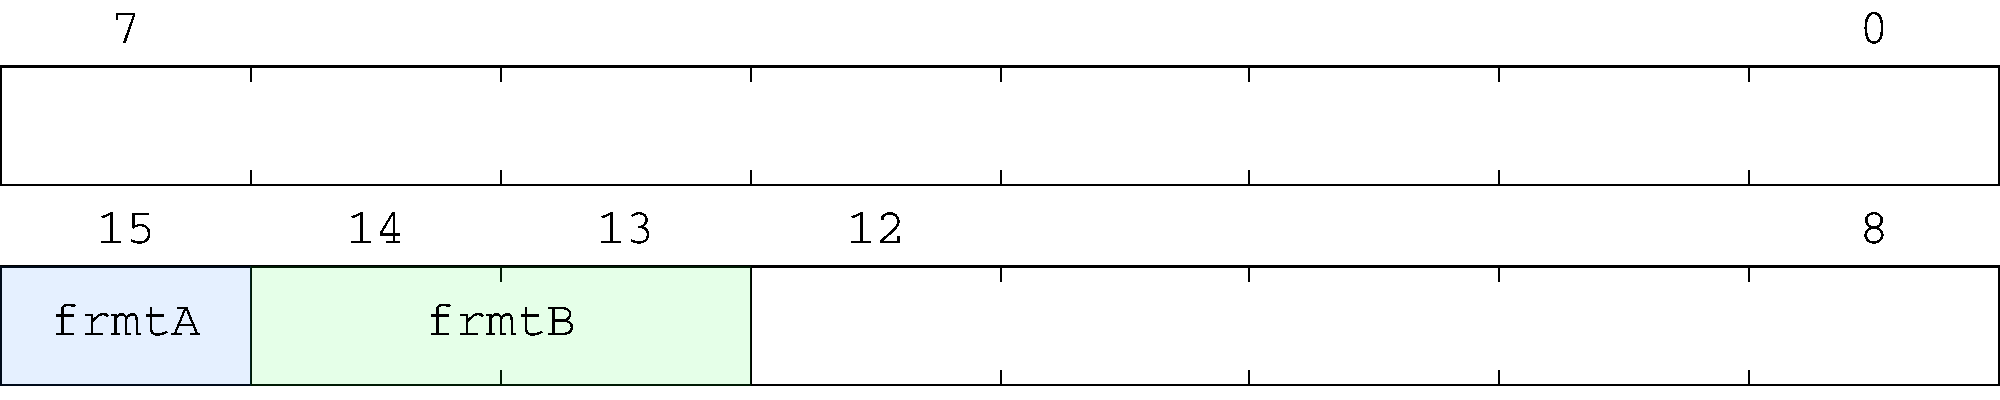
\includegraphics[width=\columnwidth]{bitfields/format4_2-lane.pdf}
    \caption{Format 4 Bitfields}
    \label{figure:format4-bitfields}
\end{figure}


\end{document}

